\documentclass[a4paper]{article}
\usepackage[dvipsnames]{xcolor}
\usepackage[top=70pt,bottom=70pt,left=48pt,right=46pt]{geometry}
\definecolor{header}{RGB}{254, 100, 11}
\definecolor{defenition}{RGB}{136, 57, 239}
\definecolor{main_title}{RGB}{30, 102, 245}
\definecolor{sub_header}{RGB}{32, 159, 181}
\usepackage[english, russian]{babel}
\usepackage[utf8]{inputenc}
\usepackage{amsmath}
\usepackage{listings}
\usepackage{graphicx}
\usepackage[colorinlistoftodos]{todonotes}
\usepackage{amsmath}

\usepackage[demo]{graphicx}% remove demo option in actual document

\title{\textcolor{main_title}{Восстановление формы поверхности по распределениям степени и угла поляриазции. <<Поляризационный>> 3D - сканер}}


\author{Шмаков Владимир Евгеньевич, Салтыкова Дарья Юрьевна \\  ФФКЭ гр. Б04-105}

\begin{document}

\maketitle
                                                                                                                                
\section*{\textcolor{header}{Введение}}

Вводим


\section*{\textcolor{header}{Теоретические сведения}}

\subsection*{\textcolor{sub_header}{Формулы Френеля}}

Пусть на плоскую неподвижную границу раздела падает плоская монохроматическая волна

\begin{equation}
\textbf{E}^{(e)} = \textbf{A} e^{i(\omega t - \bf{k_1 r})}.
\end{equation}

Из соображений симметрии следует, что отраженная и прошедшая волны

\begin{equation}
\begin{gathered}
\textbf{E}^{(r)} = \textbf{R} e^{i(\omega t - \bf{k_1^{'} r})}, \\

\textbf{E}^{(d)} = \textbf{D} e^{i(\omega t - \bf{k_2 r})}.
\end{gathered}
\end{equation}

будут также плоскими и притом той же частоты $\omega$ (равенство частот следует из линейности и однородности граничных условий).

Получим известные нам из курса Оптики формулы Френеля. Для этого разложим электрическое поле каждой вышеперчисленной волны на две составляющие: лежащую в плоскости падения и перпендикулярную к этой плоскости. 

\begin{figure}[htbp]
  \centering
  \includegraphics[width= 0.6\textwidth]{1.png}
  \caption{потом подпишу}
  \label{fig:1}
\end{figure}

Пусть $\bf{e_x, e_y, e_z}$ - единичные векторы координатных осей, а $\bf{e_1, e_1^{'}, e_2}$ - единичные векторы, лежащие в плоскости падения и перпендикулярные соответственно к падающему, отраженному и преломленному лучам. Тогда

\begin{equation}
\bf{e_1} = \frac{[e_y \bf{k_1}]}{k_1}, \text{   } \bf{e_1^{'}} = \frac{[e_y \bf{k_1^{'}}]}{k_1}, \text{     }
\bf{e_2} = \frac{[e_y \bf{k_2}]}{k_1}.
\end{equation}

Введем разложения

\begin{equation}
\begin{gathered}

\textbf{A} = A_{\perp}\bf{e_y} + A_{\parallel} \be{e_1} \\
\textbf{R} = R_{\perp}\bf{e_y} + R_{\parallel} \be{e_1^{'}} \\
\textbf{D} = D_{\perp}\bf{e_y} + D_{\parallel} \be{e_2}. 

\end{gathered}
\end{equation}

Умножим скалярно первое из этих уравнений на $\bf{e_x}$, находим

\begin{equation}
A_x = A_{\parallel}(\bf{e_1e_x}) = \frac{A_{\parallel}}{k_1}(\bf{e_x[e_yk_1]}) = \frac{A_{\parallel}}{k_1}(\bf[e_xe_y]k_1)=\frac{A_{\parallel}}{k_1}(\bf{e_zk_1}) = A_{\parallel}cos\varphi.
\end{equation}

Аналогично, $A_y = A_{\perp}, A_z = -A_{\parallel} sin\varphi. $ Тогда составляющие электрического поля на границе раздела сред (z = 0)

\begin{equation}
E_x^{(e)} = cos\varphi \cdot A_{\parallel}, \text{     } E_y^{(e)} = A_{\perp}, \text{     }
E_z^{(e)} = -sin\varphi \cdot A_{\parallel}.  
\end{equation}

Фазовые множители мы опустили, так как в любой точке границы раздела они одинаковы для всех трех волн.

Найдем магнитное поле (из $[\textbf{kH}] = -\frac{\omega}{c}\textbf{D}, \text{     } [\textbf{kE}] = \frac{\omega}{c}\textbf{B}$) и его компоненты

\begin{equation}
H_x^{(e)} = -n_1 cos\varphi \cdot A_{\perp}, \text{     } H_y^{(e)} = n_1A_{\parallel}, \text{     }
H_z^{(e)} = n_1sin\varphi \cdot A_{\perp}.  
\end{equation}

Для отраженной волны:
\begin{equation}
\begin{gathered}
E_x^{(r)} = -cos\varphi \cdot R_{\parallel}, \text{     } E_y^{(r)} = R_{\perp}, \text{     } E_z^{(r)} = -sin\varphi \cdot R_{\parallel}, \\
H_x^{(r)} = n_1 cos\varphi \cdot R_{\perp}, \text{     } H_y^{(r)} = n_1 R_{\parallel}, \text{     } H_z^{(r)} = n_1 sin\varphi \cdot R_{\perp}
\end{gathered}
\end{equation}

Для прошедшей волны:

\begin{equation}
\begin{gathered}
E_x^{(d)} = cos\psi \cdot D_{\parallel}, \text{     } E_y^{(d)} = D_{\perp}, \text{      } E_z^{(d)} = -sin\psi \cdot D_{\parallel}, \\

H_x^{(d)} = -n_2 cos\psi \cdot D_{\perp}, \text{     } H_y^{(d)} = n_2 D_{\parallel}, \text{     } H_z^{(d)} = n_2 sin\psi \cdot D_{\parallel}
\end{gathered}
\end{equation}

Для определения $R_{\perp}, R_{\parallel}, D_{\perp}, D_{\parallel}$ воспользуемся граничными условиями:

\begin{equation}
\begin{gathered}
E_x^{(e)} + E_x^{(r)} = E_x^{(d)}, \text{     } E_y^{(e)} + E_y^{(r)} = E_y^{(d)}, \\

H_x^{(e)} + H_x^{(r)} = H_x^{(d)}, \text{     } H_y^{(e)} + H_y^{(r)} = H_y^{(d)} D_{\parallel}
\end{gathered}
\end{equation}

Подставляя в них найденные выше значения, получим

\begin{equation}
\begin{gathered}
cos \varphi(A_{\parallel} - R_{\parallel}) = cos \psi \cdot D_{\parallel}, \text{     } A_{\perp} + R_{\perp} = D_{\perp}, \\

n_1 cos\varphi(A_{\perp} - R_{\perp}) = n_2 cos\psi \cdot D_{\perp}, \text{     } n_1(A_{\parallel} + R_{\parallel}) = n_2 D_{\parallel}.
\end{gathered}
\end{equation}

Отсюда получаем формулы Френеля:

\begin{equation}
\begin{gathered}

r_{\perp} = \frac{R_{\perp}}{A_{\perp}} = \frac{n_1 cos\varphi - n_2 cos\psi}{n_1 cos\varphi + n_2 cos\psi}, \text{     } 

d_{\perp} = \frac{D_{\perp}}{A_{\perp}} = \frac{2 n_1 cos\varphi}{n_1 cos\varphi + n_2 cos\psi}, \\


r_{\parallel} = \frac{R_{\parallel}}{A_{\parallel}} = \frac{n_2 cos\varphi - n_1 cos\psi}{n_2 cos\varphi + n_1 cos\psi}, \text{     }

d_{\parallel} = \frac{D_{\parallel}}{A_{\parallel}} = \frac{2 n_1 cos\varphi}{n_2 cos\varphi + n_1 cos\psi}.

\end{gathered}

\label{fresnel}
\end{equation}

Далее с помощью этих коэффициентов будут получены зависимости степени поляризации от угла падения для случаев зеркального и диффузного отражения.


Отношение отраженной энергии к энергии падающей называется коэффициентом отражения $\rho$. Так как энергия пропорциональна квадрату амплитуды, формулы (\ref{fresnel}) дают для коэффициентов отражения главных составляющих падающей волны следуюшие выражения:

\begin{equation}
\rho_{\perp} = (\frac{cos\varphi - ncos\psi}{cos\varphi + ncos\psi})^2,\text{     } \rho_{\parallel} = (\frac{ncos\varphi - cos\psi}{ncos\varphi+cos\psi})^2.
\end{equation}

Аналогично определяется коэффициент пропускания $b$ - отношение прошедшей энергии к энергии падающей.

\begin{equation}
b_{\perp} = \frac{ncos\psi}{cos\phi}(\frac{2cos\varphi}{cos\varphi + ncos\psi})^2,\text{     } b_{\parallel} = \frac{ncos\psi}{cos\phi}(\frac{2cos\varphi}{ncos\varphi+cos\psi})^2.
\end{equation}

Приведем теоретические кривые для энергетических коэффициентов прохождения и преломления.

!тут должен быть график из презы

Как видно из рисунка, в отраженном свете преимущество имеет направление электрического поля, перпендикулярное плоскости
падения, а в преломленном свете – параллельное плоскости падения. Отсюда получаем, что максимальная и минимальная интенсивность для определенной ориентации (фиксированного угла поворота поляроида относительно референсного направления - здесь мы считаем референсным вертикальное вверх) могут быть представлены как

\begin{equation}
I_{max} = \frac{\rho_{\perp}}{\rho_{\perp}+\rho{\parallel}}I_\text{з}, \text{      } I_{min} = \frac{\rho_{\parallel}}{\rho_{\perp}+\rho{\parallel}}I_\text{з},
\label{i_min_max}
\end{equation}

где $I_\text{з}$ - величина зеркальной компоненты отражения в отсутствии поляроида?? хз не поняла:( (в предположении, что нет диффузного отражения).

Как мы помним, для характеристики частично
поляризованного света вводят понятие степени поляризации $\Delta$

\begin{equation}
\Delta = \frac{I_{max} - I_{min}}{I_{max} + I_{min}}.
\label{degree}
\end{equation}

\subsection*{\textcolor{sub_header}{Зеркальное отражение}}

Отраженный свет включает в себя зеркальную и диффузную компоненты. Зеркальное отражение происходит от внешней поверхности объекта.

Из (\ref{i_min_max}) и (\ref{degree}) получаем, что степень поляризации для этого случая выглядит следующим образом:

\begin{equation}
\Delta_{\text{з}} = \frac{\rho_{\perp}(n, \varphi_i) - \rho_{\parallel}(n, \varphi_i)}{\rho_{\perp}(n, \varphi_i) + \rho_{\parallel}(n, \varphi_i)}.
\end{equation}

где $\phi_i$ - угол падения. С учетом формул для коэффициентов Френеля:

\begin{equation}
\Delta_{\text{з}} = \frac{2sin^2\varphi cos\varphi \sqrt{n^2 - sin^2\phi}}{n^2 - sin^2\varphi- n^2sin^2\varphi+2sin^4\varphi}.
\end{equation}

\subsection*{\textcolor{sub_header}{Диффузное отражение}}

Диффузное отражение происходит, когда свет как бы проникает под поверхность объекта, преломляется (будучи частично поляризованным), а затем вновь испускается (уже неполяризованный). При этом диффузно отраженный свет рассеивается равномерно по всем направлениям. 

Когда свет после вторичного испускания достигает границы поверхность-воздух, происходит процесс, аналогичный тому, что описан выше, но с коэффициентом преломления $1/n$ вместо $n$. Если "внутренний" угол падения превышает $arcsin(1/n)$, происходит полное внутреннее отражение. Иначе по закону Снеллиуса можно найти угол выхода для любого "внутреннего" угла падения, а затем вычислить коэффициент пропускания для этого угла выхода. 

\begin{figure}[htbp]
  \centering
  \includegraphics[width= 0.6\textwidth]{2.png}
  \caption{потом подпишу}
  \label{fig:2}
\end{figure}

Найдем степень поляризации для этого случая:

\begin{equation}
\Delta_{\text{д}} = \frac{b_{\parallel}(n, \varphi_i') - b_{\perp}(n, \varphi_i')}{b_{\parallel}(n, \varphi_i') + b_{\perp}(n, \varphi_i')} = \frac{\rho_{\perp}(n, \varphi_i') - \rho_{\parallel}(n, \varphi_i')}{2 - \rho_{\perp}(n, \varphi_i') - \rho_{\parallel}(n, \varphi_i')}.
\end{equation}

Перейдем к углу $\varphi_t' = \varphi$

\begin{equation}
\Delta_{\text{д}} = \frac{(n-1/n)^2 sin^2 \varphi}{2+2n^2 - (n+1/n)^2sin^2\varphi + 4cos\varphi \sqrt{n^2 - sin^2\varphi}}.
\end{equation}

\subsection*{\textcolor{sub_header}{Матрицы когерентности - описание частично поляризованного света}}

Для описания полностью поляризованного света можно использовать двумерный комплексный вектор, называемый \textcolor{defenition}{вектором Джонса}. Расположим координатные оси $x$ и $y$ в плоскости перпендикулярной волновому вектору $\vec{k}$. Составляющие вектора Джонса описывают амплитуды колебания вектора $\vec{E}$ в рассматриваемой плоскости. Например:
\begin{itemize}
    \item $(1, 0)^{T}$ - линейно поляризованный свет вдоль оси x
    \item  $(\sqrt{2} / 2, \sqrt{2} / 2)^{T}$ - линейная поляризация под углом $45$ градусов
    \item $(1, i)^{T}$ - круговая поляризация. Разность фаз между колебаниями вдоль осей $x$ и $y$ - $\Delta \phi = \pi / 2$.
\end{itemize}

\begin{figure}[htbp]
  \centering
  \includegraphics[width= 0.8\textwidth]{jones.png}
  \caption{описание полностью поляризованного света при помощи векторов Джонса.}
  \label{fig:jones_vector_examples}
\end{figure}

Джонсом также был придуман и математический аппарат для описания действия линейных оптических поляризационных систем.

Пусть линейно поляризованный свет $J = [A_x, A_y]^{T}$($A_{x}, A_{y} \in R$) падает на поляроид, ось которого коллинеарна оси $y$. Свет вышедший из поляроида описывается вектором $J = [0, A_y]^{T}$. Действие поляроида на свет можно описать матрицей Джонса, представленной на рисунке \ref{fig:polaroid_responce_matrix}.


\begin{figure}[htbp]
  \centering
  \includegraphics[width= 0.8\textwidth]{stokes_2.png}
  \caption{Использование матрицы Джонса для описания действия поляроида}
  \label{fig:polaroid_responce_matrix}
\end{figure}


\textcolor{defenition}{Матрица Джонса} - матрица 2x2, которая описывает действие линейных оптических элементов на поляризованный свет. Она позволяет описать как поляризация изменяется при прохождении через оптическую систему, которая представлена данной матрицей. 



Матрицы Джонса, описывающие действие других оптических элементов приведены на рисунке \ref{fig:jones_matricies_examples}. Прелесть матриц Джонса заключается в том, что к ним можно применять стандартные линейные операторы. Например, повёрнутый на $\theta$ поляроид описывается матрицей Джонса на которую подействовали оператором поворота: $W_{\theta} M W_{\theta}^{-1} = W_{\theta} M W_{-\theta}$(здесь $W \in R^{2 \times 2} $ - матрица поворота, $M$ - исходная матрица Джонса). 

\begin{figure}[htbp]
  \centering
  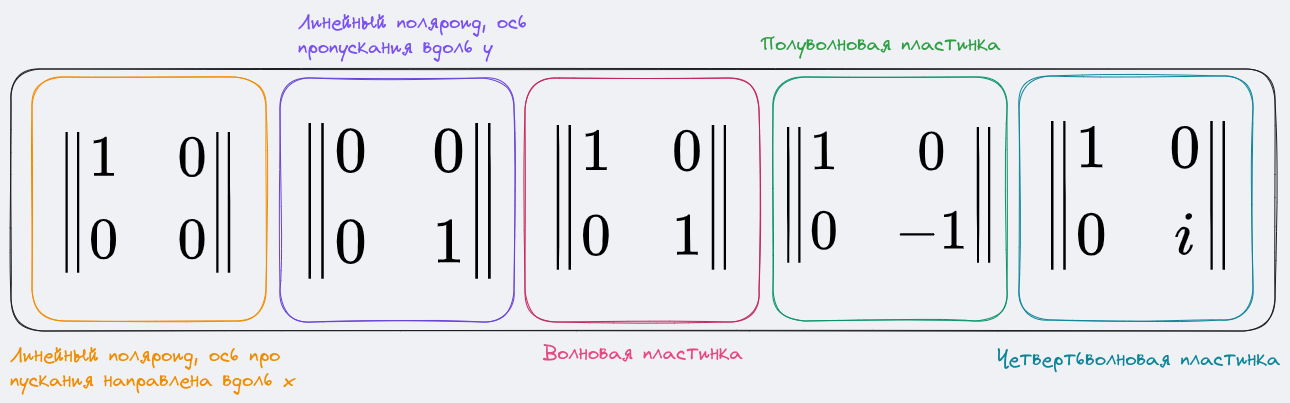
\includegraphics[width= 0.8\textwidth]{polaroid_table.png}
  \caption{Матрицы Джонса, описывающие действие линейных оптических элементов}
  \label{fig:jones_matricies_examples}
\end{figure}

Векторы Джонса не подходят для описания частично поляризованного света, ведь в данном случае $A_x$ и $A_y$ являются случайными величинами. Чтобы задать числовое описание вводят матрицу когерентности(поляризационную матрицу):

\begin{equation}\label{eqn:coherency_matrix_defenition}
    G = \begin{Vmatrix}
    \langle |E_{x}|^{2} \rangle & \langle E_{x} E_{y}^{*} \rangle \\
    \langle E_{y} E_{x}^{*} \rangle & \langle |E_{y}|^{2} \rangle
    \end{Vmatrix} = 
    \langle
        \begin{Vmatrix}
            E_{x} \\
            E_{y}
        \end{Vmatrix}
        \begin{Vmatrix}
            E_{x}^{*} & E_{y}^{*}
        \end{Vmatrix}
    \rangle
\end{equation}

На главной диагонали матрицы $G$ расположены интенсивности $I_{x}$ и $I_{y}$. Недиагональные элементы зависят от разности фаз, и амплитуд компонент волны. Они определяют поляризацию волны. 

Выведем матрицы когерентности для поляризованного света. 


\begin{equation}
G =  
\frac{1}{2}
\begin{Vmatrix} 1 \\ 0 \end{Vmatrix} 
\begin{Vmatrix} 1 & 0 \end{Vmatrix} = 
\frac{1}{2}  \begin{Vmatrix} 1 & 0\\ 0 & 0 \end{Vmatrix}
- \text{линейная поляризация вдоль оси } x
\label{x_polarized_coh_matrix}
\end{equation}

\begin{equation}
    G = \frac{1}{2} \begin{Vmatrix} 1 \\ 1 \end{Vmatrix} \begin{Vmatrix} 1 & 1 \end{Vmatrix} = \frac{1}{2}  \begin{Vmatrix} 1 & 1\\ 1 & 1 \end{Vmatrix} - \text{линейная поляризация под углом } 45 \degree
\label{45_polarized_coh_matrix}
\end{equation}

\begin{equation}
G = \frac{1}{2} \begin{Vmatrix} 1 \\ -i \end{Vmatrix} \begin{Vmatrix} 1 & i \end{Vmatrix} = \frac{1}{2}  \begin{Vmatrix} 1 & i\\ -i & 1 \end{Vmatrix} - 
\text{круговая поляризация против часовой стрелки}
\label{circ_polarized_coh_matrix}
 \end{equation}

Для естественного света все направления равновероятны. А значит $ <E_{x}> =  <E_{y}> $. Корреляции между компонентами $E_{x}$ и $E_y$ нет, а значит недиагональные элементы матрицы когерентности для естественного света равны нулю.

\begin{equation}
G = \frac{1}{2} \begin{Vmatrix}
    1 & 0 \\
    0 & 1 
\end{Vmatrix}
- \text{естественный свет}
\end{equation}

Отметим важные свойства матрицы поляризации:
\begin{itemize}
    \item $a_{ii} \in R$ - диагональные элементы матрицы являются действительными числами
    \item $a_{ij} = a_{ji}^{*}$ - транспонированная матрица поляризации является сопряженной к исходной
\end{itemize}

В силу вышеописанных свойств любая матрица поляризации может быть представлена как линейная комбинация представленная на формуле \ref{coh_matrix_as_linear_combination}.

\begin{equation}
\boxed{
    G =   
    \frac{1}{2}
    \left(
    S_{0}
    \begin{Vmatrix}
        1 & 0 \\
        0 & 1
    \end{Vmatrix}
    +
    S_{1} \begin{Vmatrix}
        1 & 0 \\
        0 & -1
    \end{Vmatrix}
    + 
    S_{2} \begin{Vmatrix}
        0 & 1 \\
        1 & 0 \\
    \end{Vmatrix}
    +
    S_{3} \begin{Vmatrix}
        0 & i \\
        -i & 0 
    \end{Vmatrix}
    \right)
    }
    \label{coh_matrix_as_linear_combination}
\end{equation}



Параметры $\begin{Vmatrix} S_{0} & S_{1} & S_{2} & S_3 \end{Vmatrix}^{T}$ называются параметрами Стокса.  


\begin{figure}[htbp]
  \centering
  \includegraphics[width= 0.8\textwidth]{stokes_phys.png.png}
  \caption{Физический смысл параметров Стокса}
  \label{fig:stokes_parametrs_examples}
\end{figure}


\begin{itemize}
    \item \textcolor{defenition}{$S_{0}$} - интенсивность света. Принято нормировать другие параметры Стокса на $S_{0}$, а $S_{0}$ принимать за единицу.
    \item \textcolor{defenition}{$S_{1}$} $\in [-1, 1]$ - Описывает степень горизонтальной или вертикальной поляризации(см рисунок \ref{fig:stokes_parametrs_examples})
    \item \textcolor{defenition}{$S_{2}$} $\in [-1, 1]$ -  Описывает по какой диагонали направлена поляризация. 
    \item \textcolor{defenition}{$S_{3}$} $\in [-1, 1]$ - Показывает направление движения вектора $\vec{E}$.
\end{itemize}



Наглядно описать состояние поляризации позволяет сфера Пуанкаре, изображенная на рисунке \ref{fig:puankare_sphere}.

\begin{figure}[htbp]
  \centering
  \includegraphics[width= 1\textwidth]{puankare_sphere.png.png}
  \caption{Состояния поляризации  на сфере Пуанкаре. Точки на сфере(синяя и красная) соответствуют полной поляризации. Фиолетовая точка - центр сферы описывает естественный свет. Оранжевая точка - частично линейно поляризованный свет.}
  \label{fig:puankare_sphere}
\end{figure}

В центре шара $S = (1 \ 0 \ 0 \ 0)^{T}$ находится естественный свет. На единичной сфере - различные состояния полностью поляризованного света. Точки внутри шара описывают частично поляризованный свет.  

Если $S_{0}$ принять равным единице, то длина вектора с началом в точке $(0 \ 0 \ 0)$ и с концом в точке описывающей данное состояние поляризации задаёт степень поляризации света(см формулу \ref{degree_of_polarization}).

\begin{equation}
    \boxed{
        \Gamma = \frac{\sqrt{S_{1}^{2} + S_{2}^{2} + S_{3}^{2}}}{S_{0}}
    }
    \label{degree_of_polarization}
\end{equation}

Линейно поляризованный свет находится на единичной окружности в плоскости $S_{3} = 0$. Чтобы узнать угол поляризации используется формула \ref{angle_of_polarization}.

\begin{equation}
    \boxed{
        \phi = \frac{1}{2}\operatorname{Arg}(S_{1} + i S_{2})
    }
    \label{angle_of_polarization}
\end{equation}



\section*{\textcolor{header}{Методика}}

\subsection*{\textcolor{sub_header}{Оборудование}}
\begin{itemize}
    \item{Поляризационная плёнка}
    \item{Сервопривод SG90}
    \item{Микроконтроллер(atmega328pb)}
    \item{Веб - камера}
    \item{Програмное обеспечение}
        \subitem{Интерпретатор python}
        \subitem{Библиотека numpy - для вычислений и матричных операций}
        \subitem{openCV - автоматизация эксперимента, обработка изображений}
        \subitem{pySerial - автоматизация эксперимента}
        \subitem{matplotlib - построение графиков, визуализация данных}
        \subitem{scipy - обработка изображений, численное разложение в ряд Фурье(алгоритм fft)}
        \subitem{Компас3D - создание экспериментальной установки}
        \subitem{arduino ide}
\end{itemize}

\subsection*{\textcolor{sub_header}{Измерение распределения степени и угла поляризации на фотографии}}

Из формул ($\ref{degree_of_polarization},\ref{angle_of_polarization}$) ясно, что для измерения степени и угла линейной поляризации достаточно измерить параметры Стокса $S_{0}, S_{1}, S_{2}$. 

Для измерения распределения трёх параметров Стокса на фотографии достаточно четырёх фотографий: 
\begin{enumerate}
    \item Разрешенное направление поляроида и ось камеры совпадают. Распределение интенсивности есть полусумма параметров $S_{0}$ и $S_{1}$.
        \begin{equation}
    M_{0} G M_{0}^{T} =
    \frac{1}{2}
    \left(
    \begin{Vmatrix}
        1 & 0 \\
        0 & 0
    \end{Vmatrix} S_{0} + 
      \begin{Vmatrix}
        1 & 0 \\
        0 & 0
    \end{Vmatrix} S_{1}
    \right)
    \to 
    J_{0} = \frac{1}{2} (S_{0} + S_{1})
    \label{0_polaroid_on_G}
\end{equation}
\item Разрешенное направление поляроида направлена под углом $45 \degree$ к оси камеры. Интенсивность есть полусумма параметров $S_{0} и S_{2}$:
\begin{equation}
    M_{45} G M_{45}^{T} =
    \frac{1}{2}
    \left(
    \frac{1}{2}
    \begin{Vmatrix}
        1 & 1 \\
        1 & 1
    \end{Vmatrix} S_{0} + 
    \frac{1}{2}
      \begin{Vmatrix}
        1 & 1 \\
        1 & 1
    \end{Vmatrix} S_{2} 
    \right)
    \to 
    J_{45} = \frac{1}{2} (S_{0} + S_{2})
    \label{45_polaroid_on_G}
\end{equation}
\item Ось камеры перпендикулярная разрешенному направлению поляроида. Интенсивность есть полуразность параметров $S_{0}$ и $S_{1}$
\begin{equation}
    M_{90} G M_{90}^{T} =
    \frac{1}{2} \left(
    \begin{Vmatrix}
        0 & 0 \\
        0 & 1
    \end{Vmatrix} S_{0} + 
      \begin{Vmatrix}
        0 & 0 \\
        0 & -1
    \end{Vmatrix} S_{1} 
    \right)
    \to 
    J_{90} = \frac{1}{2}(S_{0} - S_{1})
    \label{90_polaroid_on_G}
\end{equation}

\item Угол между разрешенным направлением и осью камеры $135 \degree$. Интенсивность есть полуразность параметров $S_{0}$ и $S_{2}$.
\begin{equation}
    M_{135} G M_{135}^{T} =
    \frac{1}{2} \left(
    \frac{1}{2}
    \begin{Vmatrix}
        1 & 1 \\
        1 & 1
    \end{Vmatrix} S_{0} -
    \frac{1}{2}
      \begin{Vmatrix}
        1 & 1 \\
        1 & 1
    \end{Vmatrix} S_{2} 
    \right)
    \to 
    J_{135} = \frac{1}{2} (S_{0} - S_{2})
    \label{135_polaroid_on_G}
\end{equation}
\end{enumerate}

\begin{minipage}{0.6\textwidth}% adapt widths of minipages to your needs

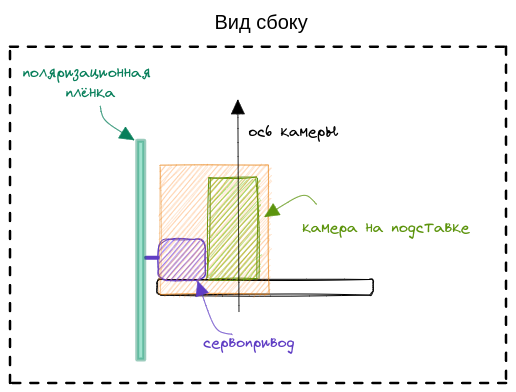
\includegraphics[width= \linewidth]{Experimental_setup.excalidraw.png}

\end{minipage}%
\hfill%
\begin{minipage}{0.4\textwidth}\raggedright
Опишем действие экспериментальной установки. Перед камерой расположена поляризационная пленка, натянутая на крестообразную основу. Центр крестообразной основы насажен на ось сервопривода, так сервопривод позволяет задавать угол между разрешенным направлением поляроида и осью камеры.
\\
Для автоматизации эксперимента используется компьютер. Общение между компьютером и микроконтроллером осуществляется по протоколу UART. Для создания снимков используется библиотека openCv.
\end{minipage}




\subsection*{\textcolor{sub_header}{Преобразование распределения степени и угла поляризации в 3D - скан объекта}}

ВОТ ТУТ ПРО ТО КАК ПОЛУЧАЕЦА КАРТА(найти про второй угол нормали)


Оказывается, что для восстановления карты высот достаточно знания карты нормалей. 

Представим карту нормалей в виде векторов вида $\vec{n}(x, y) = (p(x, y), q(x, y), 1)^{T}$. Пусть $f(x, y)$ задаёт искомую поверхность(карту высот). Тогда:
$$
p(x, y) = -\frac{\partial f}{\partial x} \hspace{20} q(x, y) = -\frac{\partial f}{\partial y}
$$

Получили систему дифференциальных уравнений в частных производных. Решение системы имеет вид:
\begin{equation}
f(x, y) = C_{0} + \int_{(x_{0}, y_{0})}^{x, y} q dx - p dy, \hspace{20} С_{0} \in \mathbb{R} \text{ - некоторая константа, задающая начальную высоту}
\label{normal_map_naive_integration}
\end{equation}

Интеграл (\ref{normal_map_naive_integration}) может быть найден численно при помощи несложного алгоритма:



\begin{enumerate}
    \item Полагаем $C_{0} = 0$. Считаем высоту в левой верхней ячейке сетки нулевой $f(0, 0) = 0$.
    \item Считаем высоту в первой колонке. Для этого численно интегрируем функцию $q(x, y)$ с шагом равным одной клеточке.
    \item Теперь мы знаем распределение высоты в первой колонке. Интегрируем функцию $p(x, y)$ по рядам.
\end{enumerate}

\begin{figure}[htbp]
  \centering
  \includegraphics[width= 0.8\textwidth]{Безымянный-2023-05-24-0140.png}
  \caption{Простой алгоритм восстановления высот из экспериментально найденных нормалей.}
  \label{fig:algos_prostoi}
\end{figure}


Описанный выше алгоритм неустойчив к шуму. Совершенный алгоритм минимизирует ошибку (\ref{error}) между экспериментально найденной картой нормалей и картой нормалей полученной дифференцированием карты высот:
\begin{equation}
    E = \iint\limits_{\text{изображение}} \left(\frac{\partial f}{\partial x}(x, y) + p(x, y) \right)^{2} + \left(\frac{\partial f}{\partial y}(x, y) + q(x, y) \right)^{2} d x d y
    \label{error}
\end{equation}

<<Оптимальный>>(для которого минимальна ошибка \ref{error}) Фурье - образ функции высот $f(x, y)$ связан с Фурье образами функций $p(x, y)$ и $q(x, y)$ при помощи выражения \ref{Forieer_transfrom}.

\begin{equation}
\hat{F} = \frac{i u P(u, v) + i v Q(u, v)}{(u + v)^{2}}
\label{Forieer_transfrom}
\end{equation}

Поэтому для нахождения карты высот необходимо сначала найти Фурье - образы функций $p$ и  $q$. После чего найти Фурье - образ искомой функции $\hat{F}$ и выполнить обратное преобразование Фурье. Реализация этого алгоритма может быть найдена в github - репозитории проекта(ссылка в приложении).

\section*{\textcolor{header}{Результаты}}

Проверим работоспосбность устройства. При помощи экспериментальной установки найдём распределение степени и угла поляризации на поверхности чашки(рисунок \ref{fig:chashka_polarization_parameters})


\begin{figure}[htbp]
  \centering
  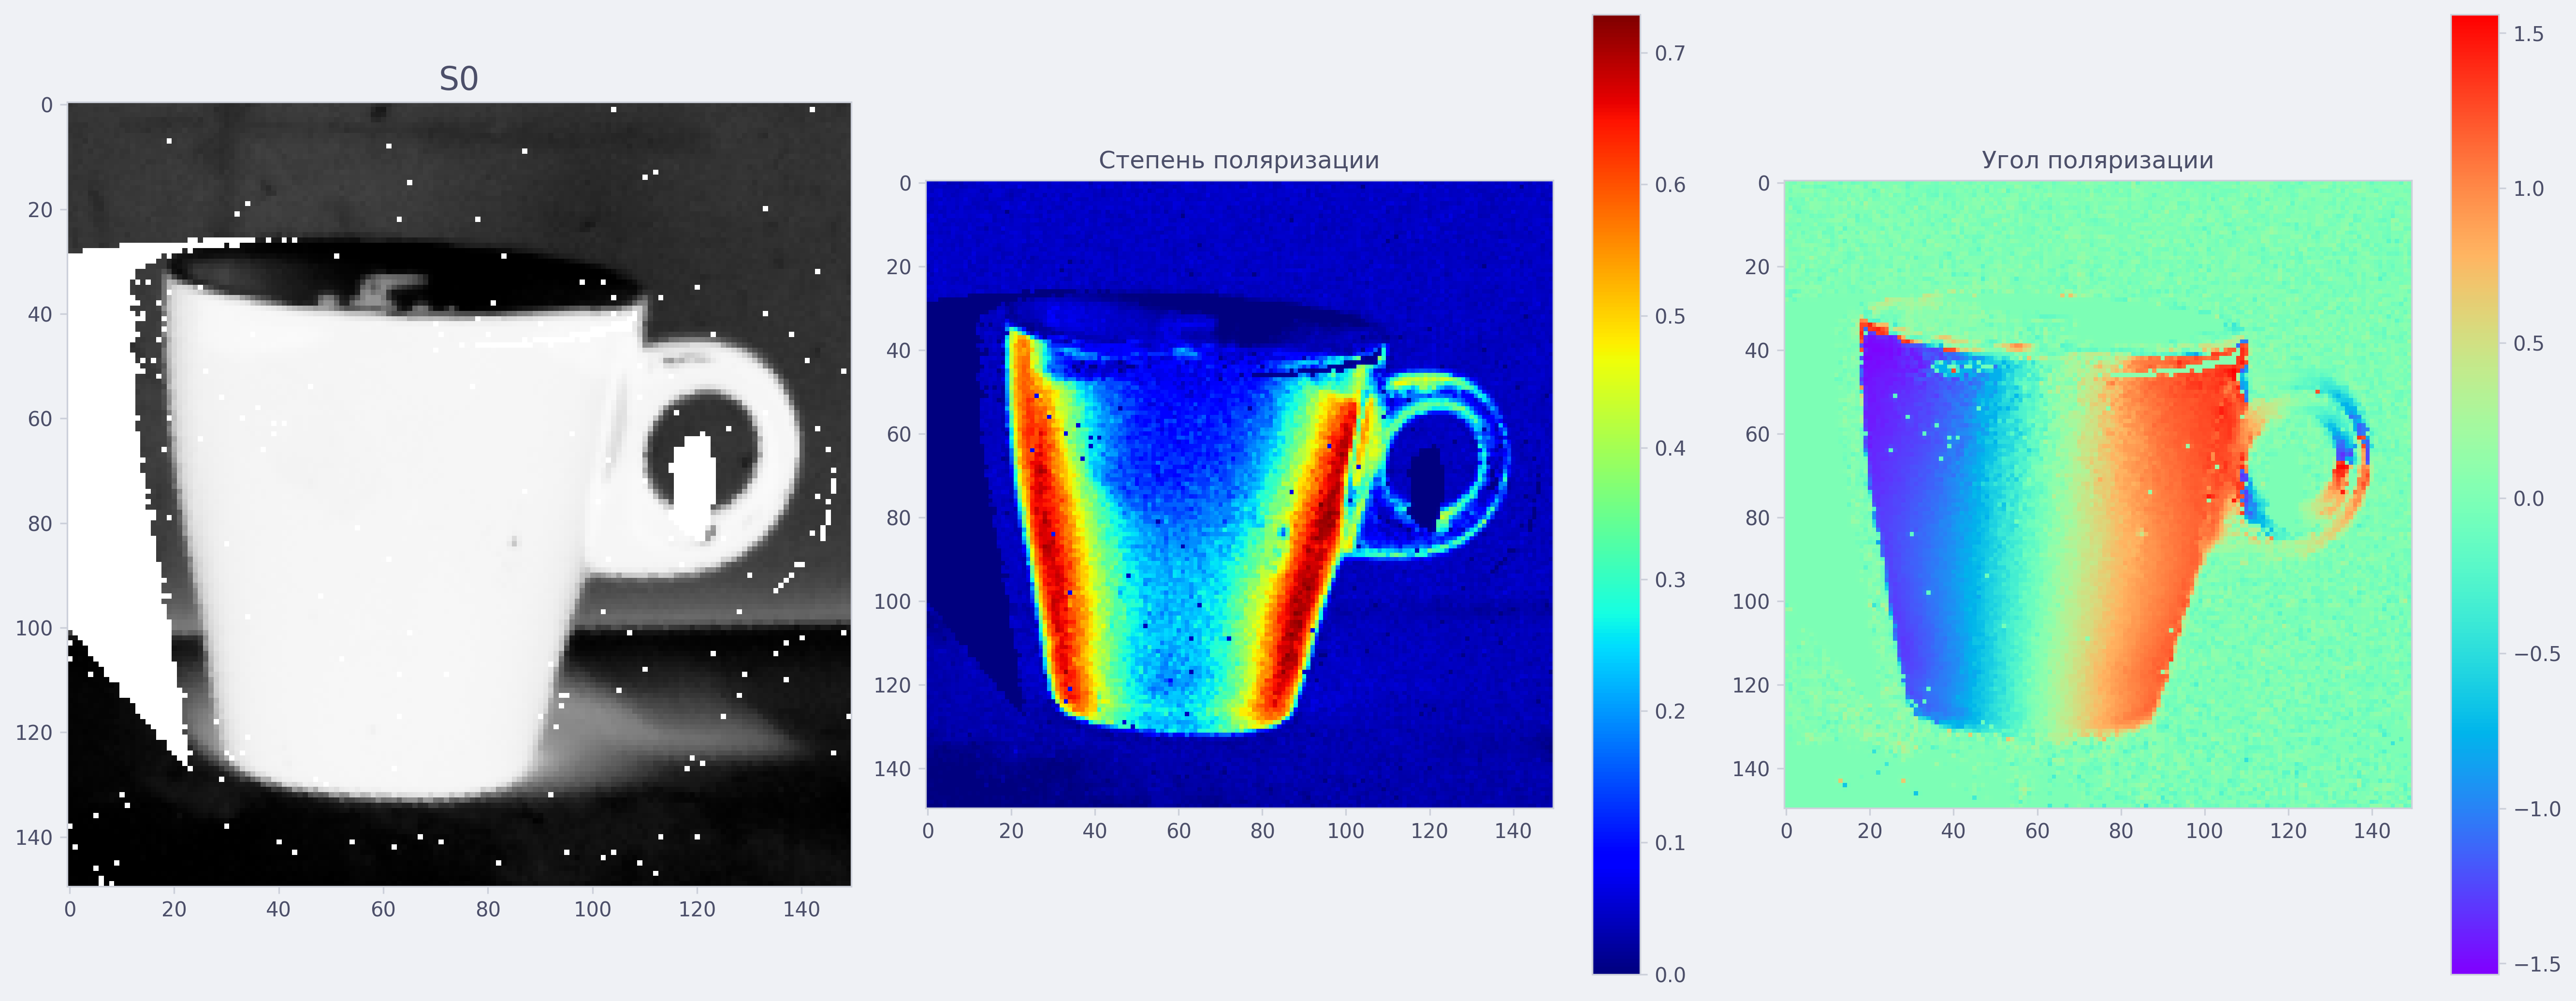
\includegraphics[width= 0.6\textwidth]{chashka_polarization_parameters.png}
  \caption{Распределение степени и угла поляризации на поверхности чашки.}
  \label{fig:chashka_polarization_parameters}
\end{figure}

При помощи описанных в методике алгоритмов восстановим форму поверхности чашки. Положим показатель преломления $n_{\text{чашка}} \sim 2$.

\begin{figure}[htbp]
  \centering
  \includegraphics[width= 0.8\textwidth]{imageedit_2_7604117862.jpg}
  \label{fig:chashka_3d}
  \caption{Восстановленная форма чашки}
\end{figure}

Похожие эксперименты были проделаны с другими объектами. 

\begin{figure}[htbp]
  \centering
  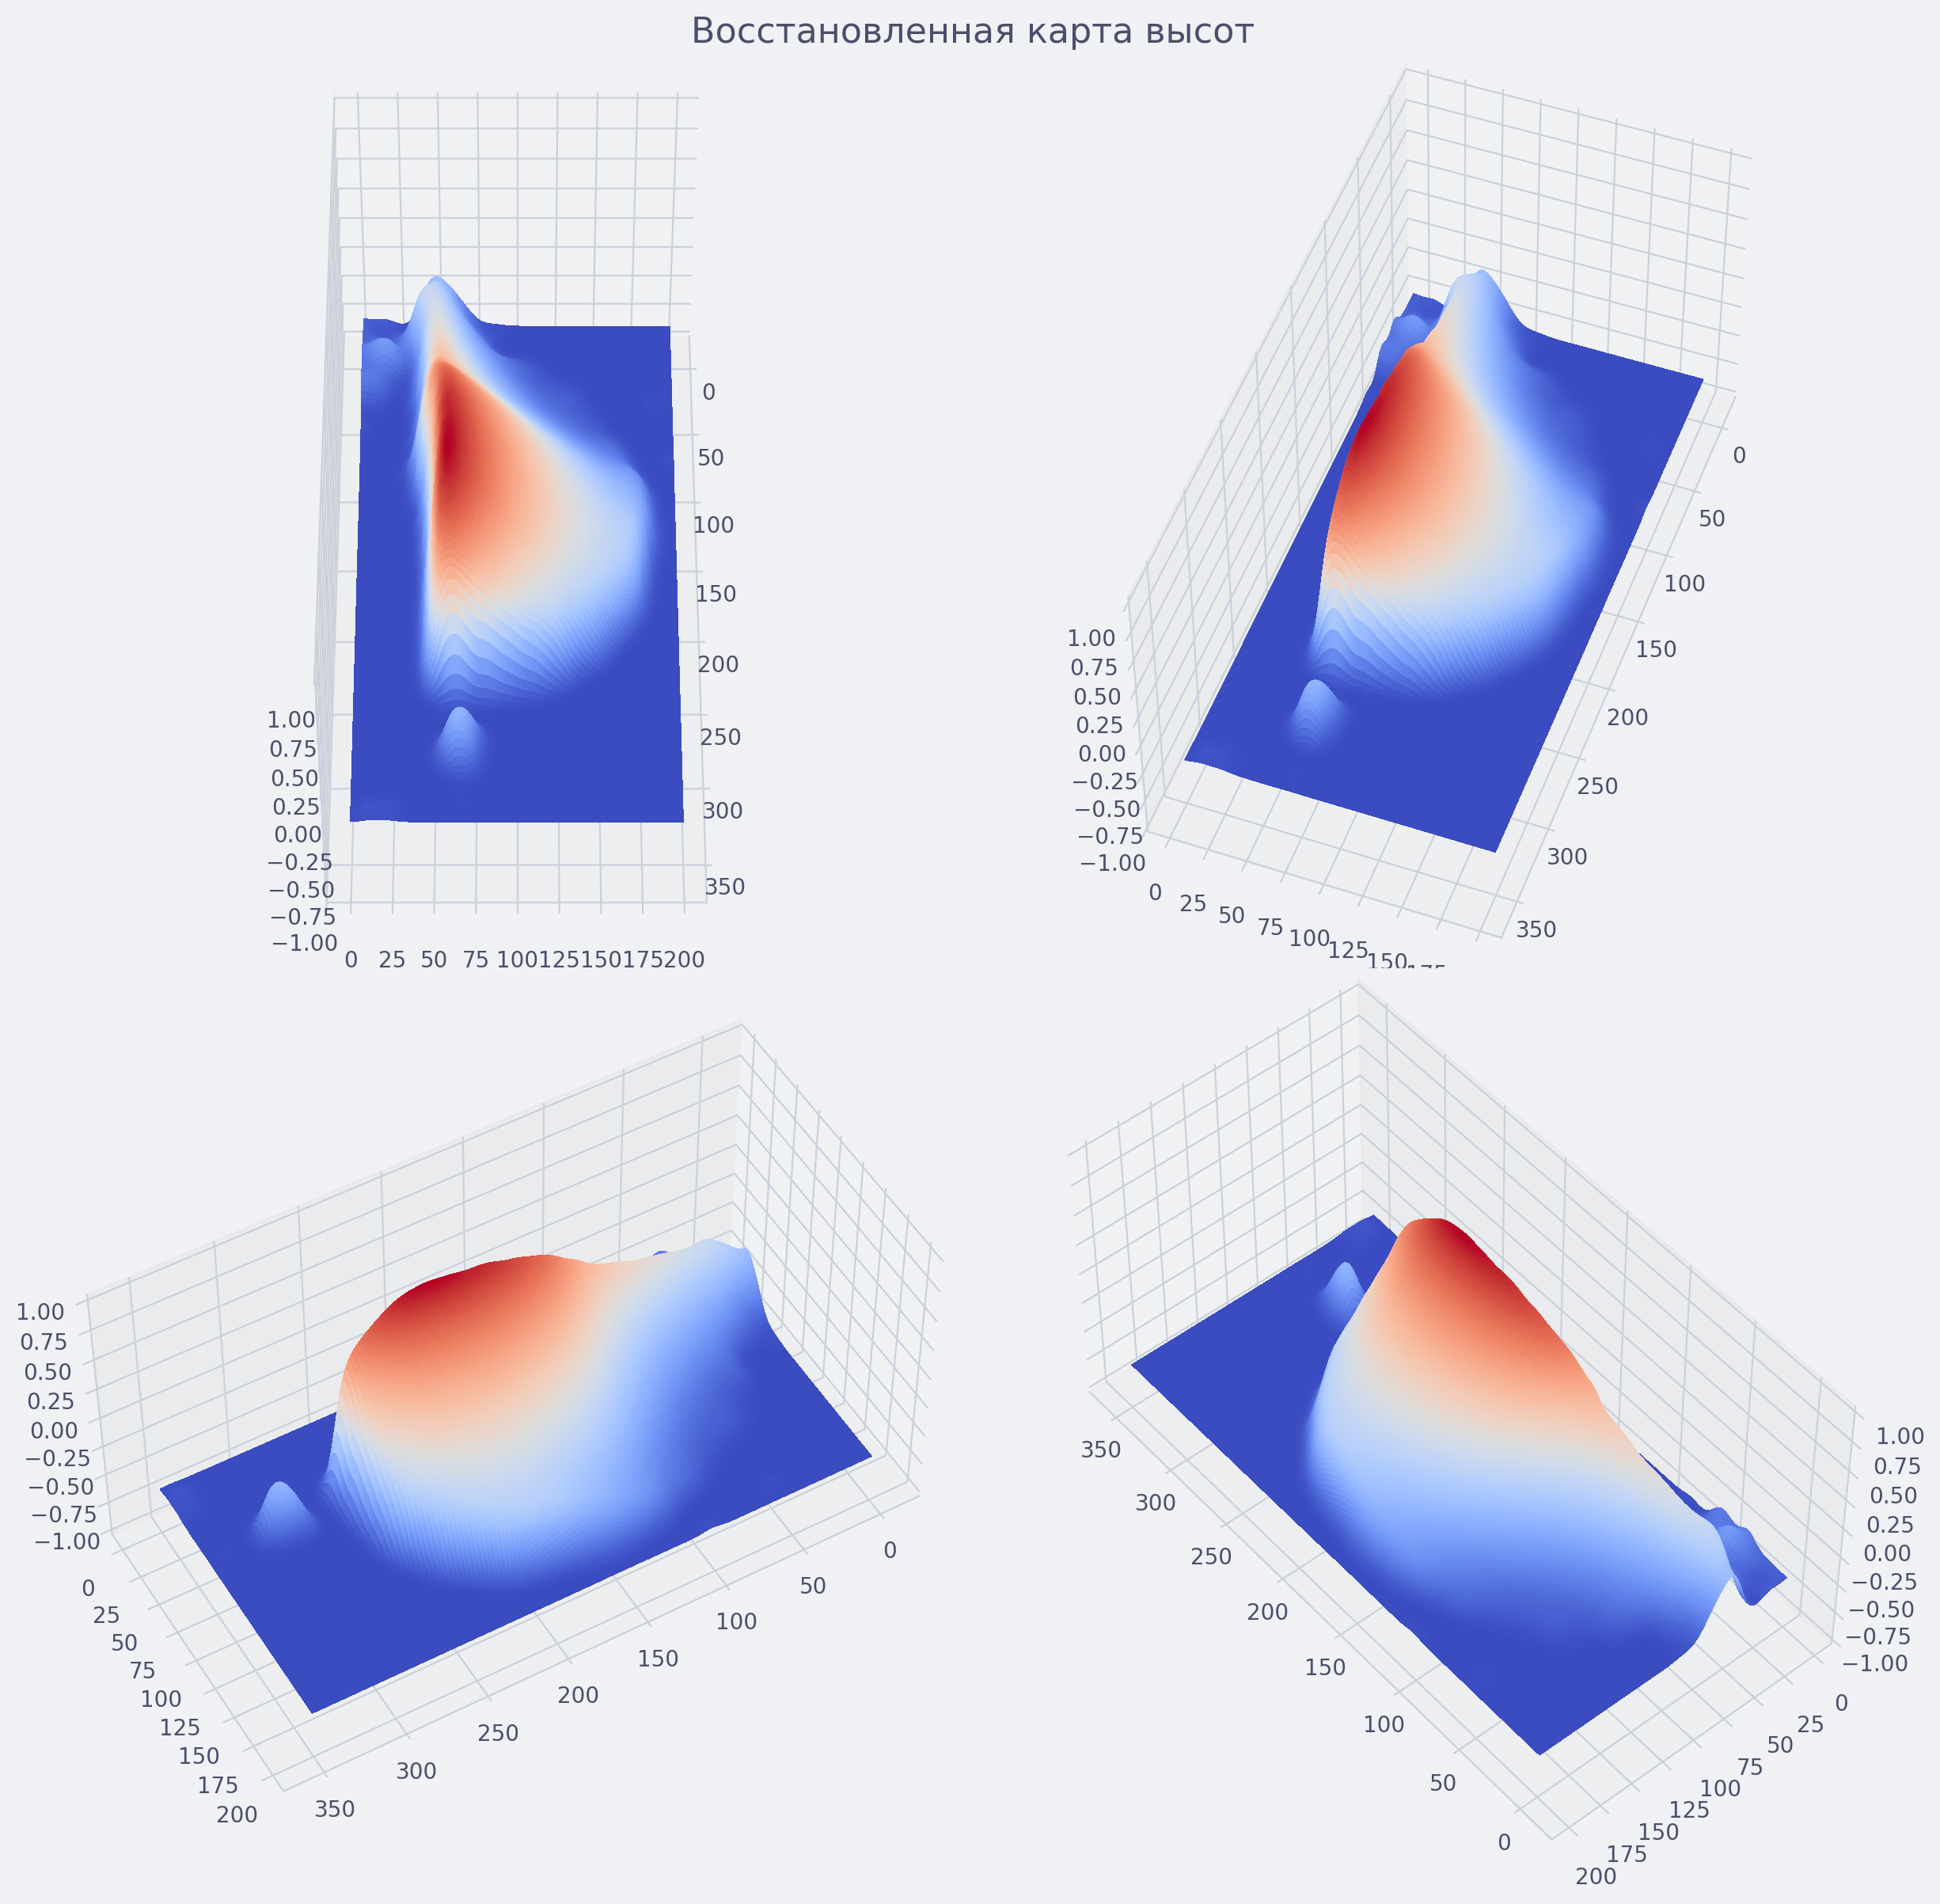
\includegraphics[width= 0.8\textwidth]{horoshiy_gorhok.png}
  \label{fig:gorshok_3d}
  \caption{Восстановленная форма цветочного горшка}
\end{figure}

Сравним точность восстановления формы. Для этого сфотографируем горшок с другого ракурса.

\section*{\textcolor{header}{Вывод}}


\end{document}